Après avoir appliqué la fonction du problème aux signaux Jardin01.mp3, Jardin02.mp3, Ville01.mp3 et MarteauPiqueur01.mp3, voici ce que nous obtenons:
\\
\\
\textbf{Légende :}
\\
\textcolor{red}{Rouge :} dépasse la durée et la puissance seuil, \textcolor{blue}{Bleu :}dépasse la puissance seuil mais plus petit que dt

\begin{figure}[htb]
\subfigure[Application sur le signal Jardin01]{
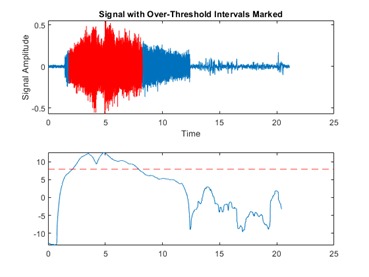
\includegraphics[width = 0.45\textwidth]{jardin01.png}
\label{Fig.sub.1.3.1}
}
\subfigure[Application sur le signal Jardin02]{
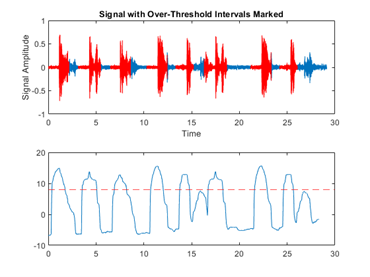
\includegraphics[width = 0.45\textwidth]{jardin02.png}
\label{Fig.sub.1.3.2}
}
\subfigure[Application sur le signal MarteauPiqueur]{
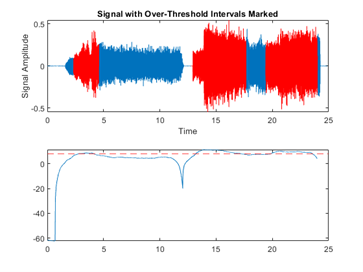
\includegraphics[width = 0.45\textwidth]{marteaaupiqueur01.png}
\label{Fig.sub.1.3.3}
}
\subfigure[Application sur le signal Ville01]{
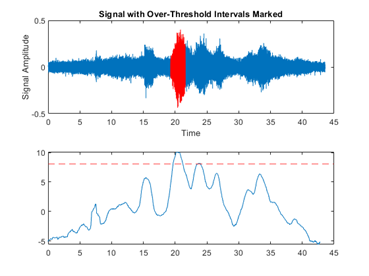
\includegraphics[width = 0.45\textwidth]{ville01.png}
\label{Fig.sub.1.3.4}
}
\caption{Application sur les signaux donnés}
\label{Fig.main.2}
\end{figure}

Pour chacun des signaux, l'amplitude en fonction du temps est présentée en haut, tandis que la puissance en dBm en fonction du temps est affichée en bas. Les pointillés rouges désignent la puissance de référence à 8 dBm et on observe bien que lorsque le signal dépasse 8 dBm et dure plus d'une seconde, on a une plage de son pénible (en rouge).
\\
\\
\begin{tabular}{|c|c|c|c|}
\hline
&
\end{tabular}
